\subsubsubsection{Communication Handling}
\subsubsubsubsection{Call Initialization}
    A session is initiated with an INVITE method which is the request from a UA client (caller). 
    INVITE has attributes containing source address, destination address, and information about the session from the caller. 
    The SIP client creates an INVITE message for callee, which is normally sent to a proxy server.

    \noindent If the OK message takes over 200ms to deliver, the progress and status (TRYING) are sent to the caller. 
    The three-way handshake occurs when the OK message confirms the connection to the caller and the ACK message confirms the existence of connection to the callee. 
    Then the media transport, which is logically separated from session initiation will be established. When there is a BYE message being sent, the session will be terminated. 

    \noindent The most common SIP messages explain for the above figure:
    \begin{itemize}
        \item \textbf {INVITE:} Initiate a dialog for establishing a call. The request is sent by a user agent client to a user agent server.
        \item \textbf {OK:} confirmation of a request.
        \item \textbf {ACK:} confirmation of the connection form caller to callee.
        \item \textbf{BYE:} Signal termination for a session and end a call.
    \end{itemize}

    \noindent Below is the illustration of a simple SIP operations:
    \begin{itemize}
        \item \textbf {Step 1:} SIP client creates INVITE message for callee, which is normally sent to a proxy server. The proxy server will then obtain the IP address of SIP server that handles requests for the requested domain. 
        \item \textbf {Step 2:} The proxy server will reference a location server to identify the next hop server. 
        \item \textbf {Step 3:} The location server (non - SIP server) stores information about the next hop server and will return the IP address of callee.
        \item \textbf {Step 4:} Trying message will be sent to the caller when the session initialization is in process.
        \item \textbf {Step 5:} When the IP address is achieved from the step 3, the proxy server will forward the INVITE message to callee machine.
        \item \textbf {Step 6 and 7:} The callee device will ring and the proxy server will forward the RINGING message from the callee to the caller.
        \item \textbf {Step 8 and 9:} When successfully reaching the callee, if the callee accepts the call, the OK response will be sent back from the callee to the caller through the proxy server.
        \item \textbf {Step 10:} An ACK confirmation will then be sent. After that a full-fledged media session is initiated between UAC and UAS. 
        \item \textbf {Step 11 and 12:} The session will then be terminated when one of two components sends the BYE message. 
    \end{itemize}

    \begin{figure}[H]
        \centering
        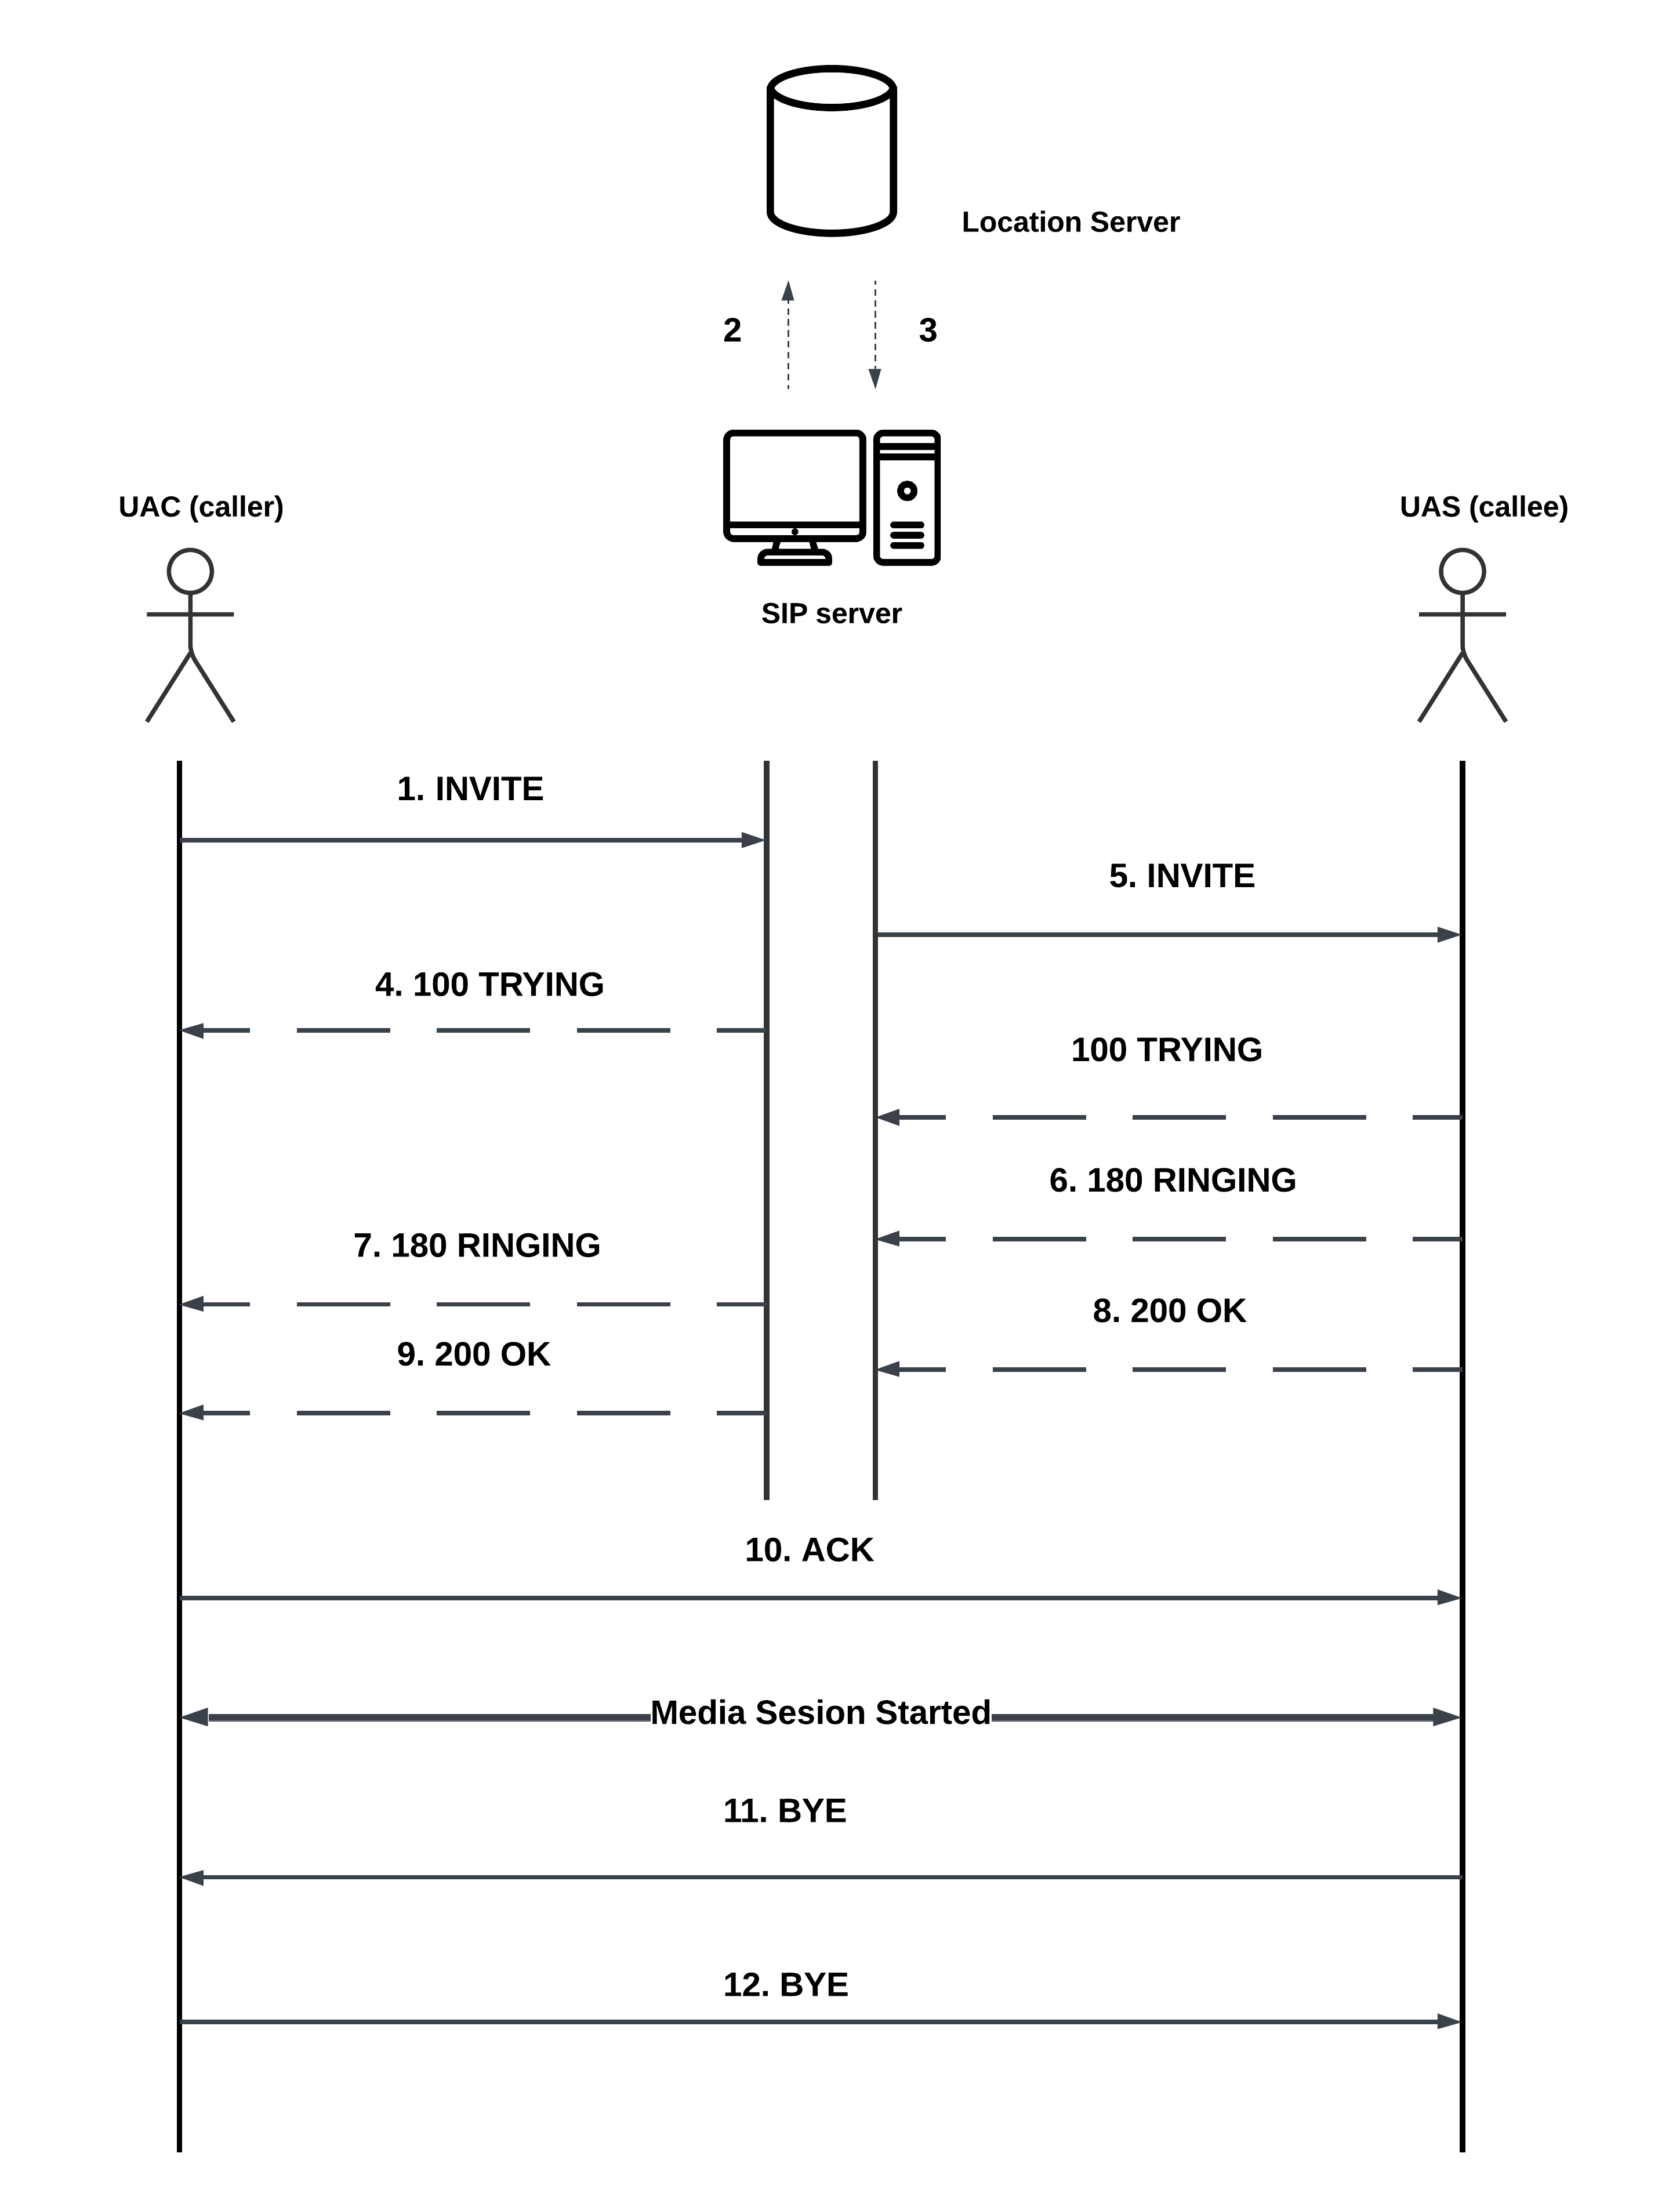
\includegraphics[width=0.7\textwidth]{image/Call Initiation.png} 
        \caption{SIP signaling and key components}
        \label{fig:sip_signaling}
    \end{figure}
    
\subsubsubsubsection{Locating the callee}
    SIP relies on supporting network services like DNS to enable the discovery of proxies and user endpoints. 
    Each user is assigned a unique SIP URI, which is essential for identification and communication. 
    To establish a call using a free SIP service, the following process is typically involved:

    \begin{itemize}
        \item \textbf{Account Registration:} A user registers an account with the free SIP service, which provides a unique SIP URI (e.g., sip: username@sip.linphone.org). 
        This registration associates the user with a proxy server, making them reachable for SIP signaling.
        \item \textbf{Call Setup:} To initiate a call, the SIP client uses the provided SIP URI and sends an INVITE message to the proxy server. 
        The proxy server relies on DNS to locate the callee's proxy server and forwards the INVITE message accordingly.
        \item \textbf{DNS Role in Call Routing:} DNS resolves the domain portion of the SIP URI (e.g., sipserver.com) to the corresponding SIP server's IP address. 
        This process ensures that the caller's proxy server can locate the appropriate next-hop server to route the call.
        \item \textbf{Communication Establishment:}  Once the proxy servers successfully exchange SIP signaling messages, the callee's user agent receives the call request, and the session is established.
    \end{itemize}

    \noindent The figure below shows the SIP registration process and how to detect the location of the callee. 
    \sloppy
    \begin{itemize}
        \item \textbf {Step 1:} One user agent with SIP URI \texttt{sip:callee\_username@sip.linphone.org} register to linphone free sip service registrar server. 
        This server stores the user’s URI and current IP address in its location service database. 
        This makes sure that the user is reachable within the \texttt{sip.linphone.org} domain. 
        \item \textbf {Step 2:} Linphone’s registrar updates its location service with the association of \texttt{sip:\allowbreak callee\_username@sip.linphone.org}.
        \item \textbf {Step 3:} Another user agent (the caller), with the SIP URI \texttt{\allowbreak sip:caller\_username\allowbreak @sip.linphone.org}, 
        sends an INVITE message to their local proxy server. 
        The destination address in the INVITE is \texttt{sip:caller\_username@sip.linphone.org}.
        \item \textbf {Step 4 and 5:} The SIP server will then query for its location service and receive the register address of the callee user agent.
        \item \textbf {Step 6:} The proxy server will then forward the INVITE method to the callee’s device. 
    \end{itemize}

    \begin{figure}[H]
        \centering
        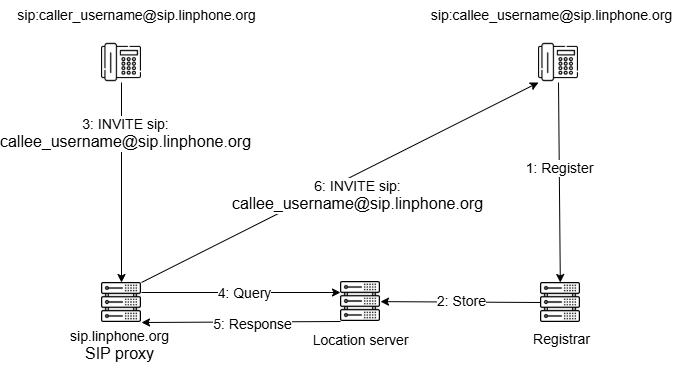
\includegraphics[width=0.7\textwidth]{image/Locating_calllee.png} 
        \caption{SIP registration and locating callee}
        \label{fig:locating_callee}
    \end{figure}

\subsubsubsubsection{One-on-One Instant Messaging}
    Instant Messaging is the process of transfering of messages between users in near real-time.
    The back and forth process to transfer messages have to be fast enough for participants to sustain an interactive dialogue.
    MESSAGE method - an extension to SIP is used to deliver messages between users. 
    The SIP MESSAGE method is ideal for asynchronous communication as it operates indepently from audio call session.
    In order to send and receive messages, client - server architecture is used.  

    \noindent One-to-one messaging is a direct exchange messages between two users. 
    After users' credentials is being checked, that information will be sent to the Flexisip server of Linphone. The Flexisip server will then create a temporary file which includes user contact list information.  
    Users can select one of the receiver among their contact lists to send a message. Message will then be sent to the receiver following these steps:

    \begin{itemize}
        \item \textbf {Initiating a message:} The sender types a message and then send it. The message will be formated into a SIP MESSAGE request. 
        \item \textbf {Message Transmission:} SIP Server will process the received SIP MESSAGE request from the sender and then forward it to the receiver. 
        \item \textbf {Receiving the message:} When the receiver get the request, Linphone will then parse the message and display it in the chat interface.
        In the case that the receiver is offline, the Flexisip server will queue the message for later delivery. A 200 OK response will be deliver to the sender to confirm sucessful exchanging messages.
    \end{itemize}

    \begin{figure}[H]
        \centering
        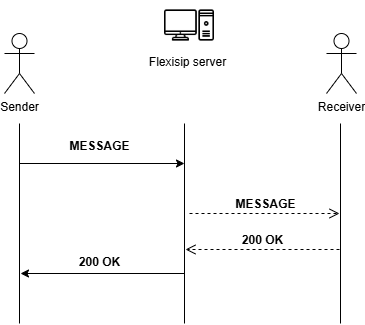
\includegraphics[width=0.5\textwidth]{image/Instant messaging.png} 
        \caption{Simple instant messaging flow}
        \label{fig:instant_messaging}
    \end{figure}


    